% Emacs settings: -*-mode: latex; TeX-master: "manual.tex"; -*-

\chapter{Inelastic scattering kernels}
\label{s:inelastic}

In this section, samples with inelastic scattering are
described. Currently, only a single sample is available that scatters
uniformly in $({\bf Q}, \omega)$ and is used for computing resolution
functions in tripple-axis instruments.

\section{Res\_sample: A uniform scatterer for resolution calculation}
\label{s:res_sample}

The component \textbf{Res\_sample} models an inelastic sample that
scatters completely homogeneous in position and energy; regardless of
the state of the incoming neutron, all directions and energies for the
scattered neutron have the same probability. This clearly does not
correspond any physically realizable samples, but the component is very
useful for computation of the resolution function and may also be used
for test and debugging purposes. The component is designed to be used
together with the \textbf{Res\_monitor} component, described in
section~\ref{s:res_monitor}.

The shape of the sample is either a hollow cylinder (like the vanadium
sample described in section~\ref{s:v_sample}) or a rectangular box. The
hollow cylinder shape is specified with inner and outer radius \textit{radius\_i}
and \textit{radius\_o} and height \textit{h}. If \textit{radius\_o} is
negative, the shape is instead a box of width \textit{radius\_i} along
the X axis, height \textit{h}, and thickness $-\textit{radius\_o}$ along the
Z axis, centered on the Z axis and with the front face in the X-Y
plane. See figure~\ref{f:res_sample}.\par
%
\begin{figure}[htbp]
  \begin{center}
        \psfrag{ri}[c][c]{\textit{radius\_i}}
        \psfrag{ro}[c][c]{\textit{radius\_o}}
        \psfrag{h}[c][c]{\textit{h}}
        \psfrag{bri}[c][c]{\textit{radius\_i}}
        \psfrag{bro}[c][c]{$-\textit{radius\_o}$}
        \psfrag{bh}[c][c]{\textit{h}}
        \psfrag{X}[c][c]{\textit{X}}
        \psfrag{Y}[c][c]{\textit{Y}}
        \psfrag{Z}[c][c]{\textit{Z}}
        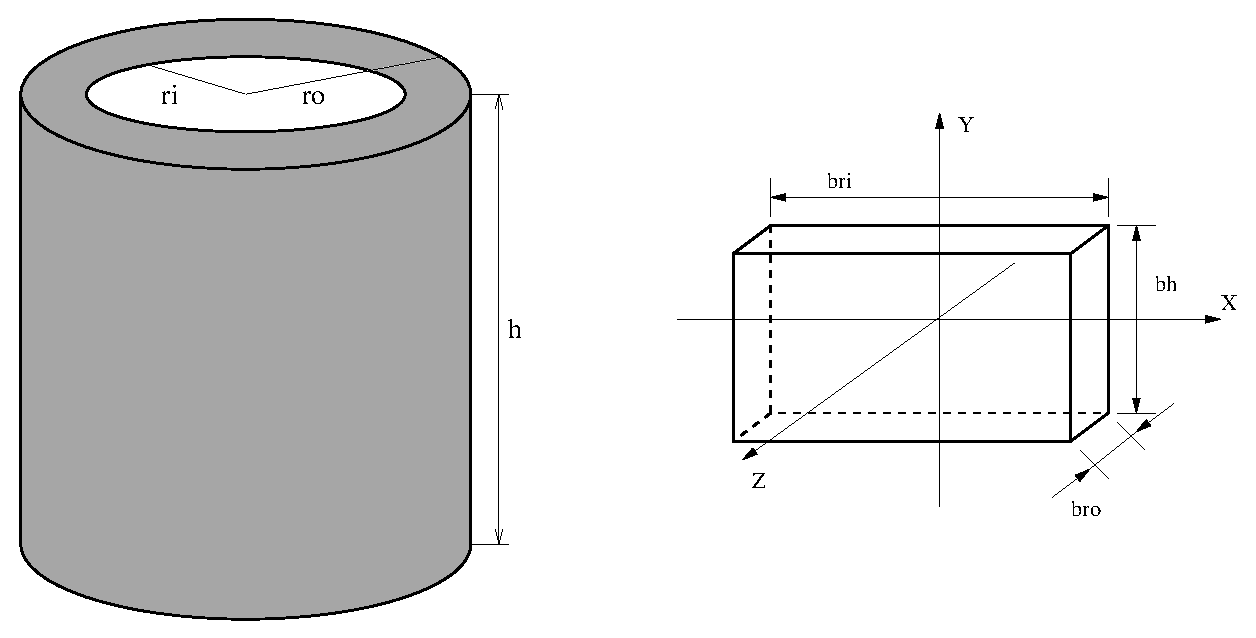
\includegraphics[width=0.9\textwidth]{figures/res_sample.eps}
    \caption{The two possible shapes of the \textbf{Res\_sample} component.}
    \label{f:res_sample}
  \end{center}
\end{figure}
%
The component only propagates the neutrons that are scattered; neutrons
that would pass through or miss the sample are absorbed. There is no
modeling of the cross section of the sample, secondary extinction
\textit{etc.}; the scattering probability is proportional to the neutron
flight path length inside the sample, with the constant of
proportionality arbitrarily set to $1/(2|\textit{radius\_o}|)$. The
reason for this is that the component is designed for computing the resolution
function of an instrument, including the sample size but independent of
any sample properties such as scattering and absorbtion cross sections.

The point of scattering in the sample is chosen at a random position
along the neutron flight path inside the sample, and the scattered
neutron is given a random energy and direction. The energy is selected in
a user-specified interval $[E_0-\Delta E; E_0+\Delta E]$ which must be
chosen large enough to cover all interesting neutrons, but preferably
not excessively large for reasons of efficiency. Similarly, the
direction is chosen in a user-specified range; the range is such that a
sphere of given center and radius is fully illuminated.

A special feature, used when computing resolution functions, is that the
component stores complete information about the scattering event in the
output parameter \textit{res\_struct}. The information includes initial
and final wave vectors, the coordinates of the scattering point, and the
neutron weight after the scattering event. From this information the
scattering parameters $({\bf Q}_i, \omega_i)$ for every scattering event
$i$ may be recorded and used to compute the resolution function of an
instrument, as explained below. For an example of how to use the
information in the output parameter, see the description of the
\textbf{Res\_monitor} component in section~\ref{s:res_monitor}.

The input parameters to the \textbf{Res\_sample} components are the
sample dimensions \textit{radius\_i}, \textit{radius\_o}, and
\textit{h}, all in meters; the center of the scattered energy range
\textit{E0} and the energy spread \textit{dE} in meV; and the target
sphere position in the local coordinate system \textit{target\_x},
\textit{target\_y}, \textit{target\_z}, and radius \textit{focus\_r}, in
meters. The only output parameter is \textit{res\_struct} containing
information about the scattering event, with all vectors given in the
local coordinate system of the component in units of meter.

\subsection{Background}

In an experiment, as well as in the simulation, the expected intensity
is by definition of the resolution function given by
%
$$
  I = \int R({\bf Q}, \omega) \sigma({\bf Q}, \omega) d{\bf Q}d\omega
$$
%
Here $I({\bf Q}_0, \omega_0)$ is the measured or simulated intensity in
the detector, $R$ is the resolution function for the instrument in a
given setup, $\sigma$ is the scattering cross section of the sample, and
$({\bf Q}, \omega)$ denote the scattering vector and energy transfer in
the sample. For the uniform scatterer, $\sigma({\bf Q}, \omega) = 1/V_0$
is a constant, so we have
%
$$
  I = 1/V_0 \int R({\bf Q}, \omega) d{\bf Q}d\omega
$$
%
If we instead consider only the intensity contributed by scattering with
parameters $({\bf Q}, \omega)$ that lie within a small part $\Delta\Omega$ of
the total phase space and has volume $\Delta V$,
%
$$
  I_{\Delta\Omega} = 1/V_0 \int_{\Delta\Omega} R({\bf Q}, \omega) d{\bf Q}d\omega
  = \frac{\Delta V}{V_0} R(\Delta\Omega)
$$
%
(where $R(\Delta\Omega)$ denotes the average value of $R$ over
$\Delta\Omega$), we get a good approximation of the value of $R$
provided that $\Delta\Omega$ is sufficiently small. This is useful with
the output from the simulations, since $I_{\Delta\Omega}$ is
approximated by

$$ I_{\Delta\Omega} \approx \sum_{({\bf Q_i},\omega_i) \in \Delta\Omega} p_i $$


This can be used to
histogram the resolution function or visualize it in different ways. The
3D visualization of the resolution function produced by the
\verb+mcresplot+ program for example uses this by displaying a cloud of
dots, the local density of which is proportional to the resolution
function.

The \verb+mcresplot+ program also computes the covariance and resolution
matrices. Letting $(x^1_i,x^2_i,x^3_i,x^4_i)$ denote the $({\bf
  Q_i},\omega_i)$ values obtained from the scattering events in the
simulation and $\mu^j = (\sum_i p_i x^j_i) / (\sum_i p_i)$ the mean
value of $x^j_i$, the covariance matrix is computed as
$$ {\bf C}_{jk} = \Big(\sum_i p_i (x^j_i - \mu_j) (x^k_i - \mu_k)\Big) /
   \Big(\sum_i p_i\Big) $$
This covariance matrix is given in the local coordinate system of the
sample component. The \verb+mcresplot+ program actually outputs the
covariance matrix in another coordinate system which is rotated around
the Y axis so that the projection to the X-Z plane of the average
scattering vector ${\bf Q}_{\rm avg} = (\sum_i p_i {\bf Q}_i) / (\sum_i
p_i)$ is parallel to the X axis.

The resolution matrix ${\bf M}$ is the inverse of the covariance matrix
and is also output in the rotated coordinate system by \verb+mcresplot+.
The 4-dimensional gaussian distribution, defined by
\begin{equation}
  \label{eq:gauss-res}
  f({\bf X}) = e^{-\frac{1}{2}{\bf X}^T {\bf M} {\bf X}}
\end{equation}
where ${\bf X} = ({\bf Q},\omega)$, has covariance matrix ${\bf C}$ and
thus defines the gaussian resolution function with the same covariance
as the resolution computed by the simulation.

The \verb+mcresplot+ program provides for the simultaneous visualization
of the computed and the gaussian resolution function by obtaining an
appropriate number of random points with the statistical
distribution~(\ref{eq:gauss-res}). Each point ${\bf X}$ is obtained as
follows: A vector ${\bf Y}$ is generated of four individually gaussian
distributed random numbers with mean zero and variance one. Using the
Cholesky decomposition of ${\bf C}$, ${\bf C} = {\bf L}{\bf L}^T$, we
have
$$ {\bf X} = {\bf L} {\bf Y}.$$



